\chapter{ODTONE}

In questo capitolo verrà descritta, analizzata e testata l'implementazione denominata ODTONE\cite{odtone}, descrivendone le funzionalità attualmente implementate ed illustrando punto per punto tutti i passaggi richiesti per compilare ed eseguire per la prima volta con successo questa implementazione, partendo direttamente dal codice disponibile presso il repository ufficiale.

\section{Descrizione}
Essa è una implementazione open-source dello standard IEEE 802.21 rilasciata con licenza LGPLv3\cite{lgpl} ed è realizzata in C++ e resa multipiattaforma tramite la libreria {\em Boost}\cite{boost}: è possibile infatti eseguire ODTONE su sistemi GNU/Linux, Windows, Android ed OpenWrt.\cite{getstart}

\section{Funzionalità implementate}

Questo progetto mira a fornire una implementazione dell'MIHF compatibile {\em out-of-the-box} con tutti i principali sistemi operativi esistenti e, di conseguenza, essendo tuttora in stato sperimentale\footnote{è attualmente disponibile la versione 0.6}, fornisce solo le funzionalità principali oppure facilmente implementabili in chiave multi-piattaforma. ODTONE è un'implementazione quasi completa, ovvero il core supporta praticamente tutto lo standard mentre i SAPs forniti, al momento della scrittura, sono solo per sistemi GNU/Linux e Windows, limitatamente per interfacce 802.3 e 802.11, e supportano solo gli eventi {\em link\_up} e {\em link\_down}.

\subsection{MIHF}
La {\em Media Independent Handover Function} fornita è composta dai tre sottocomponenti principali definiti dallo standard IEEE 802.21:
\begin{itemize}
\item {\em Media Independent Event Service} (MIES): ha il compito di vagliare gli eventi ricevuti per controllare che siano conformi allo standard e di propagarli alle entità che ne hanno richiesto la sottoscrizione. Più nel dettaglio è composto da:
\begin{itemize}
\item Event Validator: controlla che l'evento sia conforme allo standard.

\item Event Subscriber: si occupa delle sottoscrizioni agli eventi.

\item Event Publisher: si occupa di propagare gli eventi agli interessati.
\end{itemize}

\item {\em Media Independent Command Service} (MICS): ha il compito di vagliare i comandi ricevuti e di recapitarli a destinazione. Più nel dettaglio è suddiviso in:
\begin{itemize}
\item Command Validator: controlla che i comandi ricevuti siano conformi allo standard.

\item Command Publisher: propaga i comandi ai diretti interessati.
\end{itemize}

\item {\em Media Independent Command Service} (MIIS): ha il compito propagare le richieste all'IS\footnote{Information Service} e inviare indietro le risposte.
\end{itemize}

Questi componenti forniscono i servizi basilari definiti nello standard. Oltre ad essi, come rappresentato graficamente in figura \ref{fig:mihfarch}, ODTONE implementa altri componenti per fornire ulteriori funzionalità e arricchire quelle già esistenti:
\begin{itemize}
\item Service Manager: è responsabile della gestione delle richieste {\em Capability\_Discover}, le quali servono per richiedere la lista di eventi e comandi supportati dall'MIHF.

\item Communication Handler: raccoglie i messaggi ricevuti da tutti i SAPs od altre entità e li invia al modulo Service Access Controller.

\item Service Access Controller: è responsabile dell'analisi degli {\em headers} di ogni messaggio ricevuto ed al loro smistamento ai servizi interessati. La decisione è presa in base all'identificativo del tipo di messaggio ed ai {\em callbacks} registrati.

\item Link Manager: gestisce le informazioni sui Link SAPs disponibili.

\item MIH-User Manager: gestisce le informazioni su MIH-Users registrati.

\item Peer MIHF Manager: gestisce le informazioni su MIHFs remoti.

\item Transaction State Machine Controller: mantiene gli stati di ogni transazione con MIHFs remoti ed è responsabile di inviare messaggi di {\em acknowledge} ed individuare messaggi duplicati.

\end{itemize}

\begin{figure}
\centering
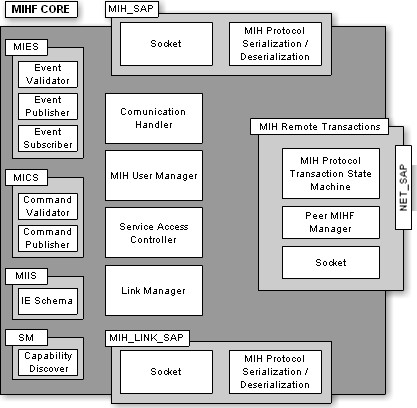
\includegraphics[]{mihfarch.jpg}
\caption{Visione concettuale dell'MIHF di ODTONE}
\label{fig:mihfarch}
\end{figure}

\subsection{MIH-Sap}
Fornisce un'astrazione {\em media-independent} per un gran numero di interfacce, ma supporta solo la generazione di eventi {\em link\_up} e {\em link\_down}. Su sistemi Linux utilizza {\em rtnetlink} e la libreria {\em libnl}\cite{libnl} per gestire le interfacce mentre su Windows utilizza le {\em SDK Libraries} ufficiali.
Le tecnologie supportate sono:
\begin{itemize}
\item IEEE 802.3
\item IEEE 802.11
\item IEEE 802.16
\item IEEE 802.20
\item IEEE 802.22
\item 3GPP GSM
\item 3GPP GPRS
\item 3GPP EDGE
\item 3GPP CDMA2000
\item 3GPP CDMA2000-HRPD
\item 3GPP UMTS
\end{itemize}

\subsection{MIH-Link-Sap 802.3}
Fornisce un SAP specifico per la tecnologia IEEE 802.3 (schematizzato in figura \ref{fig:sap3}). Supporta la generazione dei seguenti eventi:
\begin{itemize}
\item Link\_Up: generato quando viene stabilita una connessione a livello {\em datalink}, i.e. viene settato il flag {\em IF\_OPER\_UP}.
\item Link\_Down: generato quando la connessione viene interrotta, i.e. viene disattivato il flag {\em IF\_OPER\_UP}.
\item Link\_Parameters\_Report: generato in risposta ad una richiesta \\{\em Link\_Get\_Parameters}, allo scadere di un timer periodico impostabile oppure quando scatta uno dei {\em triggers} specificati con la richiesta {\em Link\_Configure\_Thresholds}. Al momento supporta solo i parametri {\em DATA\_RATE} e {\em PACKET\_ERROR\_RATE}, ottenuti tramite il comando Netlink {\em RTNL\_GET\_LINK}. Si noti che il dato sui pacchetti persi è una statistica {\em all-time}.
\end{itemize}
Supporta i seguenti comandi:
\begin{itemize}
\item Capability\_Discover: risponde con una lista di eventi e comandi supportati dal SAP.
\item Event\_Subscribe: permette di sottoscriversi agli eventi richiesti.
\item Event\_Unsubscribe: permette di annullare l'iscrizione agli eventi specificati.
\item Link\_Get\_Parameters: permette di richiedere esplicitamente l'invio di un {\em Link\_Parameters\_Report}.
\item Link\_Configure\_Thresholds: permette di configurare dei valori-soglia che quando oltrepassati faranno generare uno specifico evento.
\item Link\_Action: permette di richiedere al kernel tramite il modulo {\em if\_8023} certe operazioni sull'interfaccia. Al momento supporta solo i comandi:
\begin{itemize}
\item {\em LINK\_DISCONNECT}: richiede la disconnessione.
\item {\em LINK\_POWER\_UP}: accende l'interfaccia.
\item {\em LINK\_POWER\_DOWN}: spegne l'interfaccia.
\end{itemize}
Per poter usufruire di queste funzionalità bisogna avviare il SAP tramite un utente che abbia la capability {\em CAP\_NET\_ADMIN}, e.g. root.
\end{itemize}

\begin{figure}[h!]
\centering
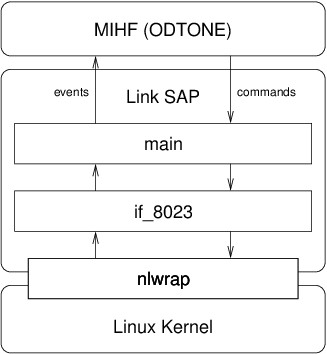
\includegraphics[scale=0.8]{sap.jpg}
\caption{Visione concettuale del Link\_SAP per 802.3}
\label{fig:sap3}
\end{figure}

\subsection{MIH-Link-Sap 802.11}
Fornisce un SAP specifico per la tecnologia IEEE 802.11. Supporta la generazione dei seguenti eventi:
\begin{itemize}
\item Link\_Detected: al termine di ogni scan delle reti 802.11 disponibili, il kernel invia un messaggio  {\em NL80211\_CMD\_NEW\_SCAN\_RESULTS}. Per ogni {\em entry} ottenuta, il SAP esegue una chiamata \\{\em NL80211\_CMD\_GET\_SCAN} per ottenere le informazioni da scrivere nell'evento.
\item Link\_Up: generato quando il modulo {\em if\_80211} riceve l'evento \\{\em NL80211\_CMD\_CONNECT} dal kernel.
\item Link\_Down: generato quando il modulo {\em if\_80211} riceve l'evento \\{\em NL80211\_CMD\_DISCONNECT} dal kernel.
\item Link\_Parameters\_Report: generato in risposta ad una richiesta \\{\em Link\_Get\_Parameters}, allo scadere di un timer periodico impostabile oppure quando scatta uno dei {\em triggers} specificati con la richiesta {\em Link\_Configure\_Thresholds}. Al momento supporta i parametri \\{\em DATA\_RATE}, {\em PACKET\_ERROR\_RATE} e {\em SIGNAL\_STRENGTH}, ottenuti tramite il comando Netlink {\em RTNL\_GET\_LINK}. Si noti che il dato sui pacchetti persi è una statistica {\em all-time} e {\em SIGNAL\_STRENGTH} non è altro che l'RSSI.
\end{itemize}
Supporta i seguenti comandi:
\begin{itemize}
\item Capability\_Discover: risponde con una lista di eventi e comandi supportati dal SAP.
\item Event\_Subscribe: permette di sottoscriversi agli eventi richiesti.
\item Event\_Unsubscribe: permette di annullare l'iscrizione agli eventi specificati.
\item Link\_Get\_Parameters: permette di richiedere esplicitamente l'invio di un {\em Link\_Parameters\_Report}.
\item Link\_Configure\_Thresholds: permette di configurare dei valori-soglia che quando oltrepassati faranno generare uno specifico evento.
\item Link\_Action: permette di richiedere al kernel tramite il modulo {\em if\_80211} certe operazioni sull'interfaccia. Al momento supporta i comandi:

\begin{itemize}
\item {\em LINK\_DISCONNECT}: richiede la disconnessione.

\item {\em LINK\_POWER\_UP}: accende l'interfaccia.

\item {\em LINK\_POWER\_DOWN}: spegne l'interfaccia.

\item {\em LINK\_LOW\_POWER}: mette l'interfaccia in modalità a basso consumo energetico. (non supportato da vecchie versioni del kernel)

\item {\em LINK\_SCAN}: richiede esplicitamente uno scan della reti Wi-Fi disponibili.

\end{itemize}
Per poter usufruire di queste funzionalità bisogna avviare il SAP tramite un utente che abbia la capability {\em CAP\_NET\_ADMIN}, e.g. root.
\end{itemize}

\subsection{La libreria libodtone}
Per poter scrivere un programma che interagisca con l'MIHF, quindi un MIH-User oppure un SAP, è possibile utilizzare la libreria inclusa {\em libodtone}, la quale fornisce tutte le funzioni necessarie per comunicare correttamente con il core: è disponibile come unica libreria solo dalla versione 0.6 di ODTONE ed è l'unione delle precedenti librerie 'base', 'mih', 'sap' e 'net'\cite{changelog}. Fornisce tutte le classi {\em helper} necessarie per facilitare lo sviluppo delle applicazioni utente, come servizi di debug, gestione di liste, log, gestione delle eccezioni e generazione di numeri pseudo-casuali. Definisce inoltre tutti i tipi di dato del protocollo MIH specificati nello standard e fornisce delle classi per facilitare la creazione dei messaggi, il loro {\em parsing}, la loro ricezione ed il loro l'invio. Per gli ultimi due, i servizi sono implementati sulla base della classe della libreria Boost {\em boost::asio} che fornisce comunicazione tramite I/O asincrono, unica tipologia di comunicazione offerta dalla libreria: è necessario infatti eseguire qualsiasi operazione asincronicamente, registrando gli opportuni {\em callbacks} tramite la funzione {\em boost::bind()}.

\section{Compilazione ed esecuzione}
Vengono di seguito illustrati tutti i passaggi per compilare ed eseguire per la prima volta ODTONE recuperando il codice dal repository ufficiale su un sistema Debian\cite{debian} {\em Wheezy}.

\subsection{Compilazione}
La procedura per compilare ODTONE dal repository ufficiale è la seguente (al momento c'è un problema con le dipendenze da risolvere manualmente\cite{snapshot}):
\begin{enumerate}

\item prelevare la prima parte di dipendenze necessarie:\\
\cmdroot{apt-get update}
\cmdroot{apt-get install build-essential git realpath cmake autoconf \\automake libboost-all-dev}

\item prelevare l'ultima versione:\\
\cmduser{git clone https://github.com/ATNoG/ODTONE.git odtone}

\item prelevare i sottomoduli:\\
\cmduser{git submodule update --init}

\item passare momentaneamente al ramo {\em testing} di Debian:\\
\cmdroot{vi /etc/apt/sources.list}
e sostituire la parola {\em stable} o {\em wheezy} in {\em testing}, e.g.:\\
\cmd{deb http://mi.mirror.garr.it/mirrors/debian/ testing main}

\item prelevare la seconda parte di dipendenze necessarie:\\
\cmdroot{apt-get update}
\cmdroot{apt-get install librdf0-dev libnl-3-dev \\libnl-route-3-dev libnl-genl-3-dev}

\item ritornare al ramo {\em stable} di Debian:\\
\cmdroot{vi /etc/apt/sources.list}
e.g.:\\
\cmd{deb http://mi.mirror.garr.it/mirrors/debian/ stable main}

\item procedere alla compilazione:\\
\cmduser{cd odtone}
\cmduser{cmake .}
\cmduser{make -j2}

\end{enumerate}

\subsection{Esecuzione}

Appena finita la compilazione, è necessario rendere disponibili le librerie appena compilate al sistema.

\begin{enumerate}

\item creare dei links simbolici in /usr/lib:\\
\cmdroot{ln -s \$(realpath lib/odtone/libodtone.so) \\/usr/lib/libodtone.so.0.5}
\cmdroot{ln -s \$(realpath lib/external/libnl/nlwrap/libnlwrap.so) \\/usr/lib/libnlwrap.so.0.5}

\item eseguire per primo l'MIHF:\\
\cmduser{./src/mihf/odtone-mihf}

\item eseguire un SAP per ogni interfaccia, inserendo l'indirizzo MAC appropriato:

802.11:\\
\cmdroot{./app/sap\_80211\_linux/odtone-sap\_80211 \\-{}-link.link\_addr <MAC>}

802.3:\\
\cmdroot{./app/sap\_8023/odtone-sap\_8023 -{}-link.link\_addr <MAC>}

\item infine eseguire l'MIH-User d'esempio fornito:\\
\cmduser{./app/mih\_usr/odtone-mih\_usr -{}-dest mihf1}

\end{enumerate}

Una volta che ogni componente sarà avviato, è possibile eseguire l'MIH-User che invierà una richiesta {\em capability\_discover} per sapere quali interfacce sono disponibili e, per ognuna di queste, una richiesta di sottoscrizione. Ora è possibile scollegarsi dalla rete wireless oppure staccare fisicamente il cavo CAT5 per veder l'MIH-User ricevere l'evento {\em link\_down} e segnalarlo su {\em stdout}. Una volta ripristinato il collegamento, vedremo l'MIH-User ricevere un evento {\em link\_up}. Per realizzare il programma MIH-proxy, descritto nel prossimo capitolo, è stato utilizzato come base per il codice l'MIH-User ufficiale.

\section{Risoluzione problemi}
Può capitare che la compilazione non vada a buon fine per degli errori della libreria Boost. In tal caso bisogna modificare il file xtime.hpp della libreria Boost:\\
\cmdroot{vi /usr/include/boost/thread/xtime.hpp}
sostituendo "TIME\_UTC" con "TIME\_UTC\_":\\
\begin{minted}[mathescape,linenos,numbersep=5pt,gobble=0,frame=lines,framesep=1mm]{diff}
--- xtime.hpp   2014-02-18 03:26:56.291068347 +0100
+++ xtime1.hpp  2014-02-18 03:27:23.679204146 +0100
@@ -20,7 +20,7 @@

 enum xtime_clock_types
 {
-    TIME_UTC=1
+    TIME_UTC_=1
 //    TIME_TAI,
 //    TIME_MONOTONIC,
 //    TIME_PROCESS,
\end{minted}

Per quanto riguarda l'esecuzione, se dobbiamo eseguire più istanze dello stesso SAP, bisogna modificare il file .conf contenuto nella directory dove si trova l'eseguibile assegnando differenti indirizzi per distinguere l'istanza del SAP e differenti porte su cui mettersi in ascolto per la ricezione di messaggi dall'MIHF.

\section{Sviluppi futuri}
Per quanto riguarda lo sviluppo di ODTONE, la priorità maggiore rimane arricchire l'insieme dei SAPs disponibili poiché ufficialmente viene fornito un SAP generico per tutte le interfacce, ma che supporta solo gli eventi {\em link\_up} e {\em link\_down}, e dei LINK\_SAP specifici solo per 802.3 e 802.11 per sistemi Linux e Windows. Bisogna quindi completare il lavoro implementando il supporto per altre tecnologie, specialmente per la famiglia 3GPP, e completare la lista di comandi ed eventi supportati da ogni SAP.